\documentclass[9pt]{exam} 
\footer{}{}{}
\addpoints
\pointsinmargin

\usepackage[fleqn]{amsmath}
\usepackage{amssymb} %standard classy maths symbols
\usepackage[a4paper, margin=1in]{geometry} %makes it easy to specify where to put stuff on the page

\usepackage{tcolorbox} % basic but good package for boxes around text
\tcbset{colback=black!5!white}

\usepackage{tikz} % interval diagrams, sets, etc.

\begin{document}

\textbf{Name:} \dotfill

\begin{center}
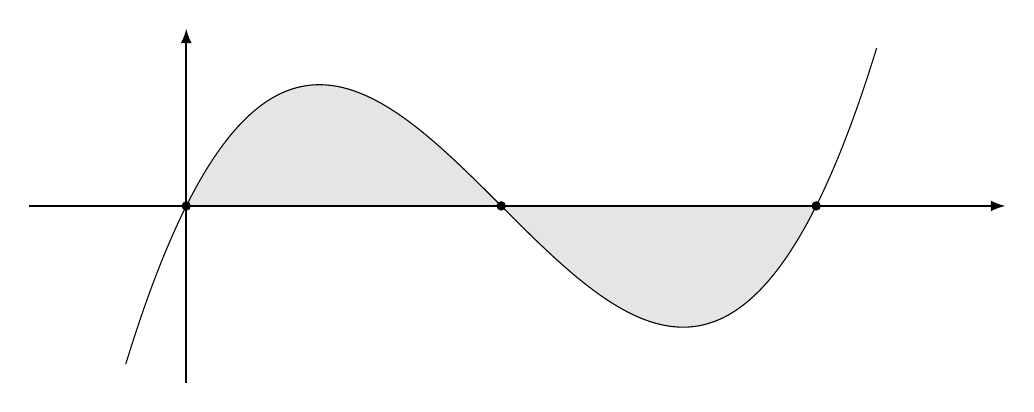
\begin{tikzpicture}[yscale=0.5, xscale=2]

  % Shade the two lobes between x=0 and x=4
  \fill[gray!20]
    (0,0) -- plot[domain=0:2, samples=200] (\x, {\x*(\x-2)*(\x-4)}) -- (2,0) -- cycle;
  \fill[gray!20]
    (2,0) -- plot[domain=2:4, samples=200] (\x, {\x*(\x-2)*(\x-4)}) -- (4,0) -- cycle;
    
  % Axes (no ticks/labels)
  \draw[thick, -latex] (-1,0) -- (5.2,0) ;
  \draw[thick, -latex] (0,-4.5) -- (0,4.5) ;

  % The cubic curve on [-1,5]
  \clip (-1, -4) rectangle (5, 4);
  \draw[smooth, domain=-1:5, samples=200]
    plot (\x, {\x*(\x-2)*(\x-4)});
    
   \fill[black] (0,0) ellipse (0.03 and 0.12);
   \fill[black] (2,0) ellipse (0.03 and 0.12);
   \fill[black] (4,0) ellipse (0.03 and 0.12);
   
\end{tikzpicture}
\end{center}

\begin{questions}

\question[1] Label the zeros on the graph of $f(x)= x(x-2)(x-4)$ above. \hfill (We use this $f$ below as well.)

\question[1] Like in first year, use distributivity to give the fully expanded form of $f(x)$.
\fillwithdottedlines{3cm}


\question[3]
Find the antiderivative of $f$.
\fillwithdottedlines{3cm}


\question[4] Compute the shaded area on the graph above.
\fillwithdottedlines{\stretch{1}}


\question[0] \textbf{Bonus.}  
Compute $ \int \tfrac 12 \cos(x) \sin(x)^3 - 3 \cos(x) \sin(x)^2 + 4 \cos(x) \sin(x) \, dx$.

\end{questions}


\begin{tcolorbox}

\textbf{Name of marker:}

\begin{center}
\gradetable[h][questions]
\end{center}

\end{tcolorbox}


\end{document}